\chapter{System Architecture}

\noindent Figure~\ref{fig:architecture} illustrates the system architecture for the ASTRO Platform, designed to support small-scale vendors by facilitating bulk order discounts, demand forecasting, and logistics optimisation. This architecture provides a clear overview of the platform’s components and how they work together to streamline the entire process from order initiation to optimized delivery.

\begin{figure}[h]
    \centering
    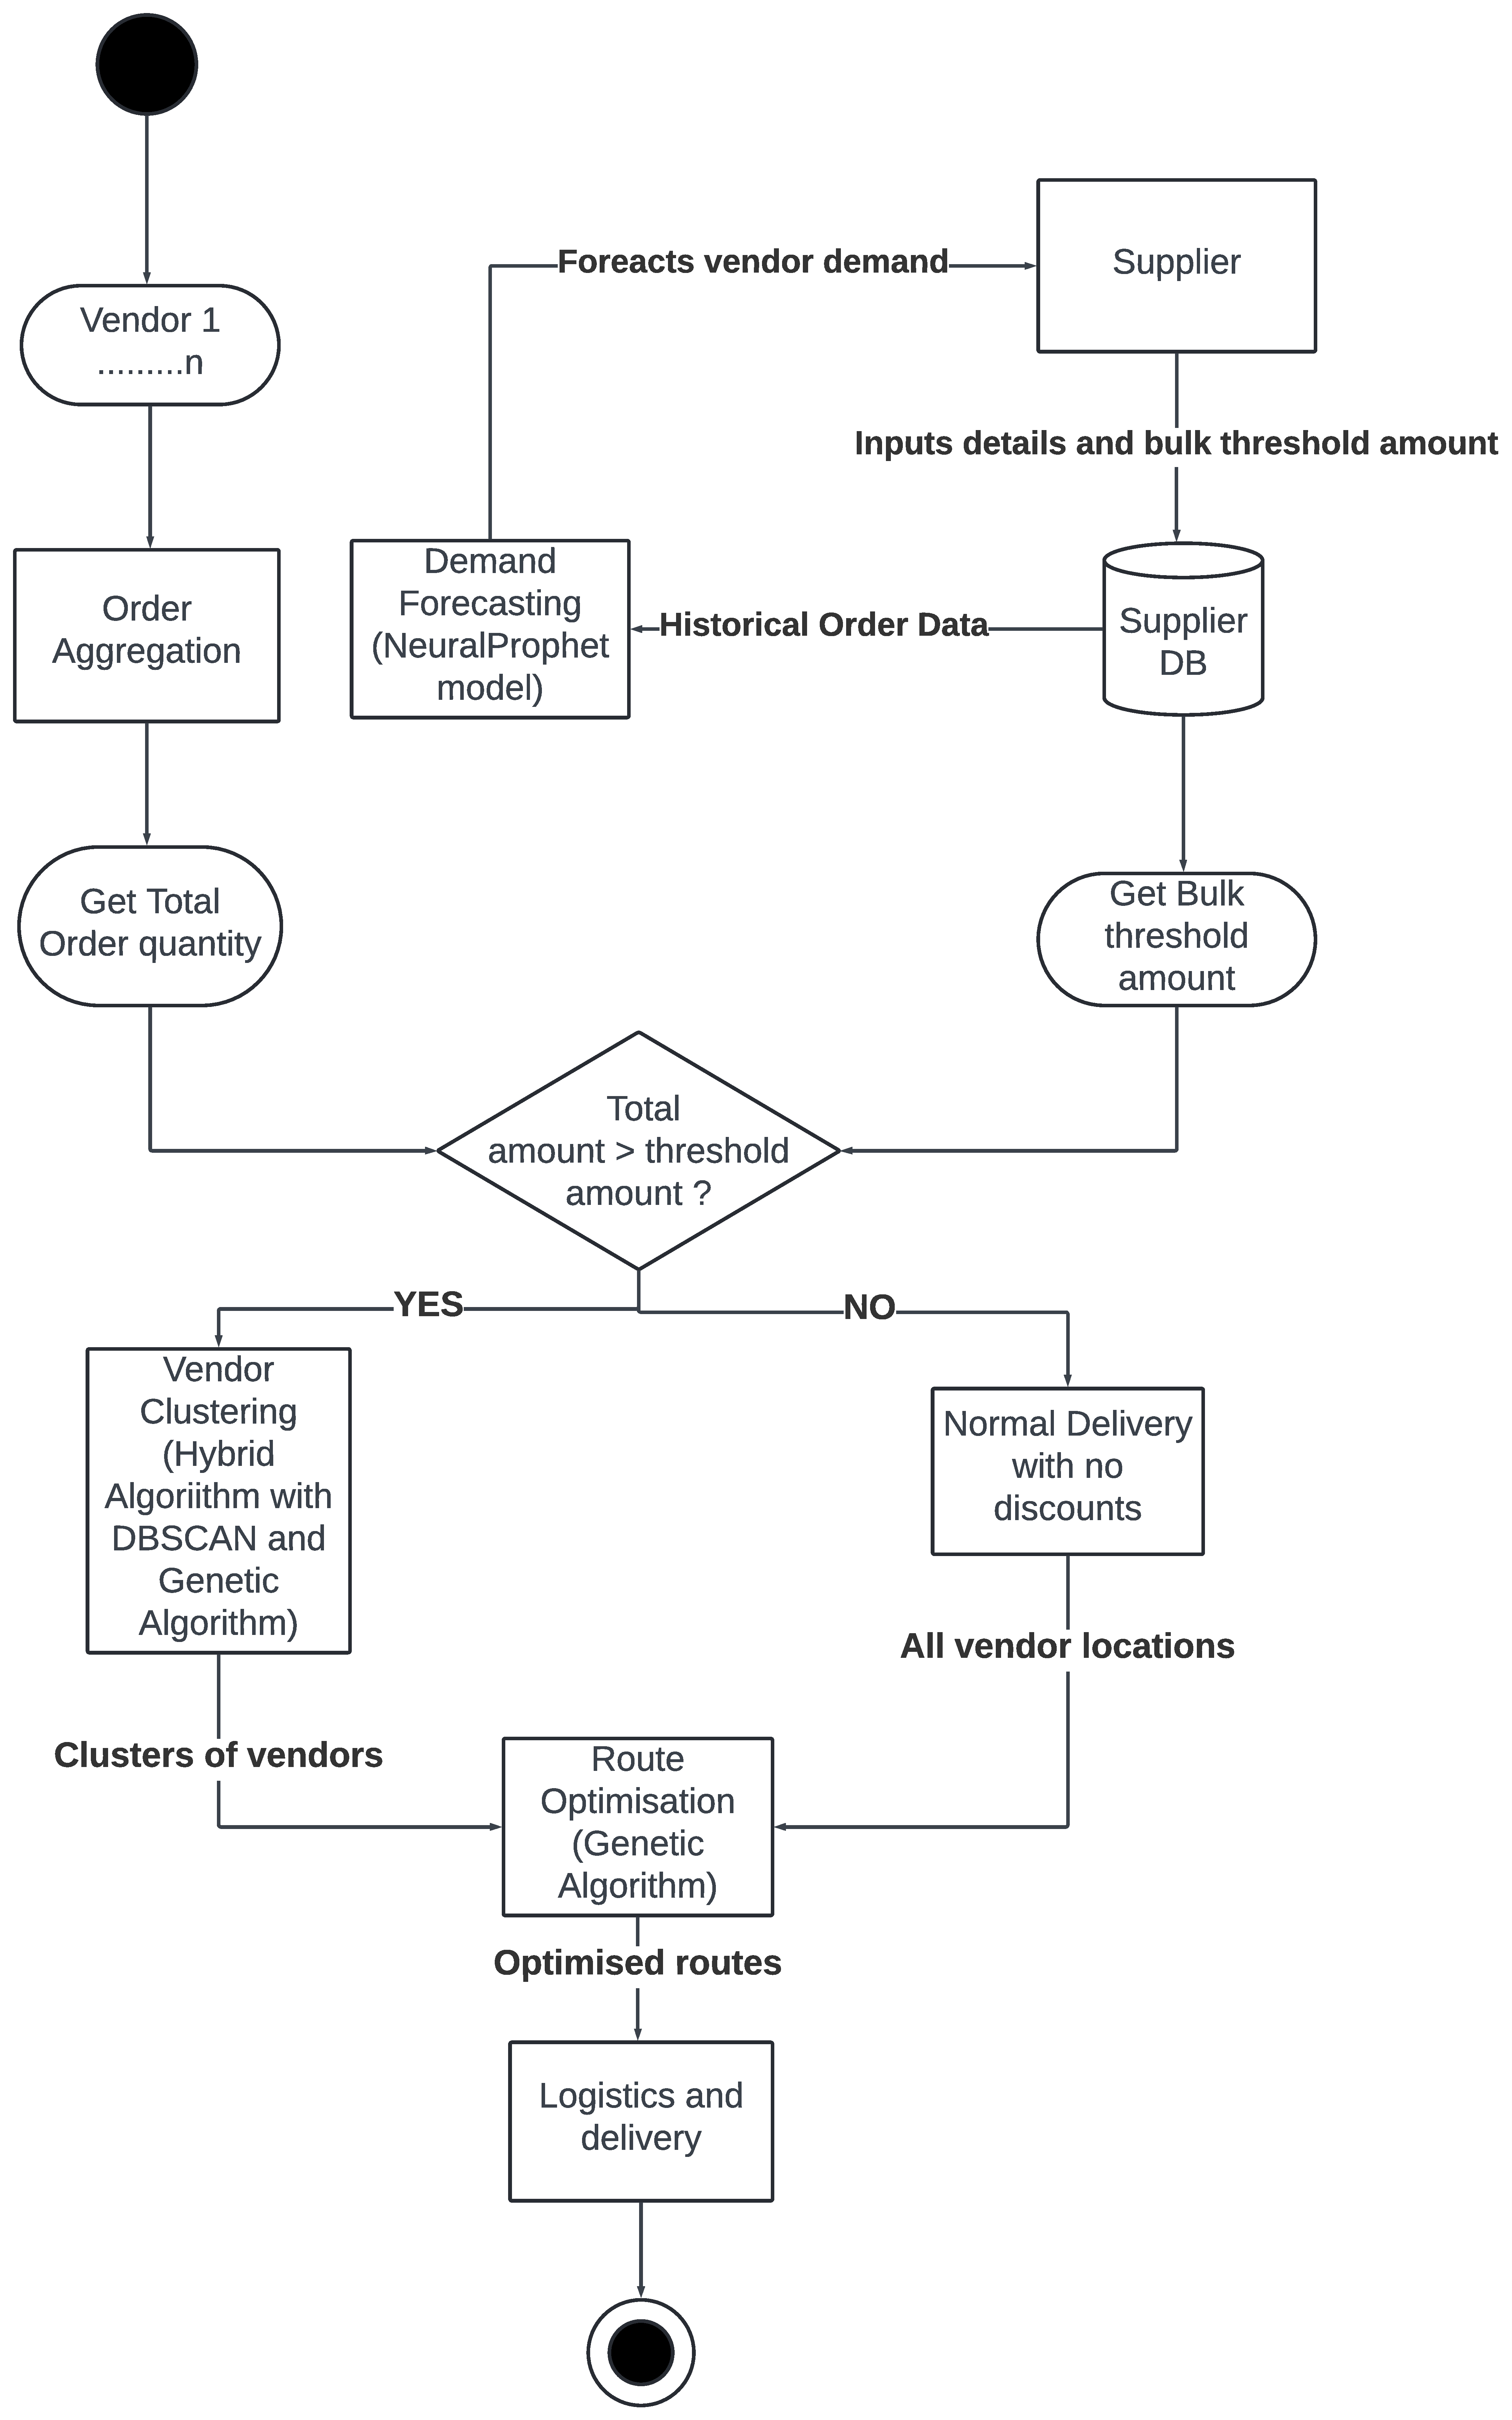
\includegraphics[width=0.5\textwidth]{Figures/sys_arch.pdf}
    \caption{System Architecture}
    \label{fig:architecture}
\end{figure}

\par The system as shown in Fig.~\ref{fig:architecture} is composed of multiple modules, each designed to enhance specific functions of the supply chain process. The Order Aggregation Module is responsible for grouping similar orders from multiple vendors to facilitate bulk purchasing. The Vendor Clustering Module applies machine learning techniques to identify optimal clusters of vendors based on their order patterns and geographic locations. The Route Optimization Module determines the most efficient delivery paths by selecting from multiple algorithms based on the number of vendors in a cluster. The Logistics and Delivery Module ensures the smooth execution of deliveries by incorporating real-time tracking and optimized scheduling. Lastly, the Demand Forecasting Module analyzes historical order data to predict future demand trends, enabling better decision-making for suppliers and reducing the risks of overstocking or understocking. The system also includes a Supplier Management Module, which allows suppliers to define bulk discount thresholds and manage product availability


\section{Vendor Clustering Module}

The Order Aggregation Module builds on the insights provided by the demand forecasting module. Once multiple vendors agree to participate in a joint order, this module combines their requirements into a single bulk order. The process ensures that the MOQ thresholds are met, unlocking discounts from suppliers that would be unattainable for individual vendors.

The aggregation process also categorizes and organizes the joint order to ensure that products are distributed efficiently. Each vendor's share of the bulk order is clearly delineated, and the aggregated data serves as input for the subsequent logistics operations.

Notifications play a key role in this module: vendors are informed about the opportunity to join an order and, once confirmed, receive updates about the order status and expected delivery timelines. The module ensures transparency and coordination among vendors, simplifying the process of collective purchasing.

\section{Route Optimisation Module}

The Route Optimisation Module is responsible for ensuring efficient delivery of the aggregated orders. After the order is finalized and fulfilled by the supplier, this module uses Green Route Optimisation algorithms to design an optimal delivery route.

Since the joint order often involves multiple vendors located in different areas, the Route optimisation module focuses on clustering delivery locations and minimizing logistics costs. The Route Flexibility and Service Time Window feature ensures that deliveries are scheduled efficiently while adhering to time constraints.

The module optimizes the route for a single vehicle tasked with delivering products to multiple vendors. Factors such as load capacity, distance between vendors, and delivery time windows are considered to achieve the most cost-effective and eco-friendly route. By reducing unnecessary travel and fuel consumption, this module contributes to both financial savings and environmental sustainability.

\section{Demand Forecasting Module}

The Demand Forecasting Module lies at the heart of the platform, enabling vendors to predict future sales and order cycles. By analysing historical sales data, the module leverages the Neural Prophet model to identify trends, seasonal patterns, and demand fluctuations. The predictions provide vendors with actionable insights into when and how much to order, ensuring they maintain optimal inventory levels while avoiding overstocking or stockouts.

Additionally, this module facilitates order cycle prediction, which is critical for synchronizing vendor orders. When a vendor places an order with a supplier, the platform uses the demand forecasting output to identify similar demand cycles for other vendors. This allows the platform to notify these vendors about the opportunity to join the order, achieving the Minimum Order Quantity (MOQ) threshold required for bulk discounts. By doing so, the demand forecasting module not only supports individual vendors but also sets the foundation for collective collaboration.


The seamless integration of demand forecasting, order aggregation, and route optimisation modules creates a powerful, collaborative platform that addresses the challenges faced by small-scale vendors. The demand forecasting module drives proactive order management, the order aggregation module facilitates cost-effective purchasing, and the route optimisation module ensures efficient delivery. Together, these modules enable vendors to compete with large retail chains by reducing costs, improving operations, and fostering a cooperative ecosystem.
